\pagebreak
\subsection{Task 1 - Building a VMware Environment}
For this demonstration secure data centre environment setup, I installed ESXi inside VMware Workstation 12 on my University of South Wales Applied Cyber Security designated workstation. This allowed me to use a single physical machine to manage and screenshot (via VMware's `Print Screen' functionality) the ESXi installation directly, manage the servers installed inside ESXi via the vSphere Web Client and vSphere Client (desktop), and test the configuration from a Windows 10 Enterprise client that was also installed inside VMware Workstation 12.

In a real-world deployment of ESXi, it would be installed bare-metal -- in other words, ESXi would be installed directly onto the physical hardware as the primary Operating System and would then be managed remotely for the most part.

\bigskip
\noindent The process for building the VMware environment is as follows:

\subsubsection*{Download the vSphere environment software}
\begin{enumerate}[series=task1methodology]
  \item Download the vSphere environment from the \textit{OnTheHub\textsuperscript{\textregistered}} website\footnote{\url{https://onthehub.com/}}.
\end{enumerate}

\noindent From Figure~\ref{fig:task1:01_downloadvsphere} in the \nameref{app:ancillaryscreenshots} appendix, it shows that three pieces of software are available for download. \todo{Detail confusion because of the `update' iso - this is actually only ESXi 6.0.0 and I erroneously installed it.}

\subsubsection*{Create a new virtual machine in VMware Workstation}
\begin{enumerate}[resume*=task1methodology]
  \item Create a new virtual machine for ESXi in VMware Workstation 12. Notable steps:
    \begin{enumerate}[label=\alph*)]
      \item Select the ESXi ISO in the `Guest Operating System Installation' step.
        % \begin{minipage}{\linewidth}
        \begin{figure}[H]
          \centering
          \captionsetup{skip=2pt}
          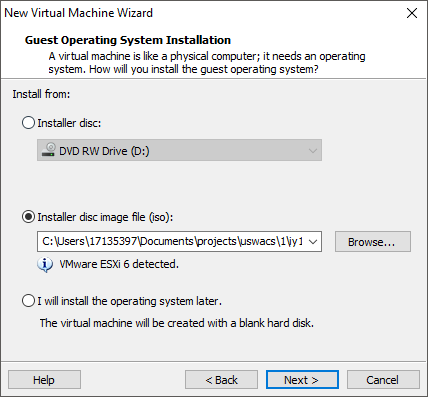
\includegraphics{task1_02_vmwareinstall_02}
          \caption{Selecting the ESXi ISO for installation into the new VM}
          \label{fig:task1:02_vmwarewiz_02}
        \end{figure}
        % \end{minipage}
      \item Increase the `Number of processors' and `Number of cores per processor' in the `Processor Configuration' step because several VMs will be running within this ESXi VM.
        \begin{figure}[H]
          \centering
          \captionsetup{skip=2pt}
          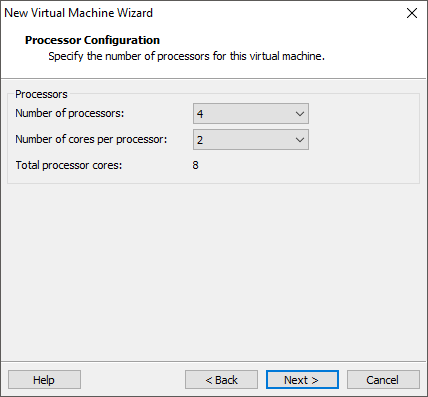
\includegraphics{task1_02_vmwareinstall_03}
          \caption{Increasing the number of processors for the ESXi VM}
          \label{fig:task1:02_vmwarewiz_03}
        \end{figure}
      \item Increase the amount of memory allocated to the ESXi VM in the `Memory for the Virtual Machine' step as because several VMs will be running within this ESXi VM. With consideration of the failover configuration of Task 2 \todo{ref this}, I decided to give the VM 16GB of memory. This would allow each of the 4 VMs inside ESXi \textit{(2 servers and a failover for each)} to have 4GB of memory.
        \begin{figure}[H]
          \centering
          \captionsetup{skip=2pt}
          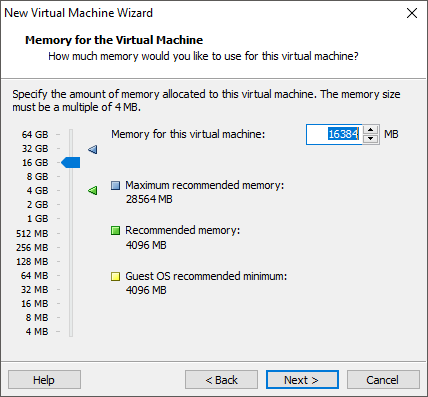
\includegraphics{task1_02_vmwareinstall_04}
          \caption{Increasing the amount of memory for the ESXi VM}
          \label{fig:task1:02_vmwarewiz_04}
        \end{figure}
      \item Setup the `Host-only Network' only in the `Network Type' step. I will add the `NAT Adapter' later and demonstrate how to configure ESXi to use it correctly at that time.
        \begin{figure}[H]
          \centering
          \captionsetup{skip=2pt}
          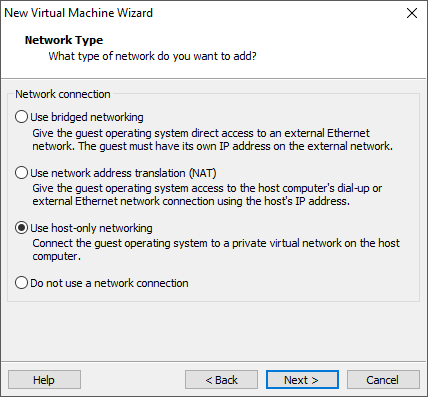
\includegraphics{task1_02_vmwareinstall_05}
          \caption{Configuring the initial network adapter for the VM}
          \label{fig:task1:02_vmwarewiz_05}
        \end{figure}
      \item Increase the maximum disk size in the `Specify Disk Capacity' step to 200GB. This will allow each of the VMs inside ESXi to have 40GB of space for 4x40=160GB of VMs and then 40GB extra for ESXi to use for storing the server install ISO, snapshots, et cetera.
        \begin{figure}[H]
          \centering
          \captionsetup{skip=2pt}
          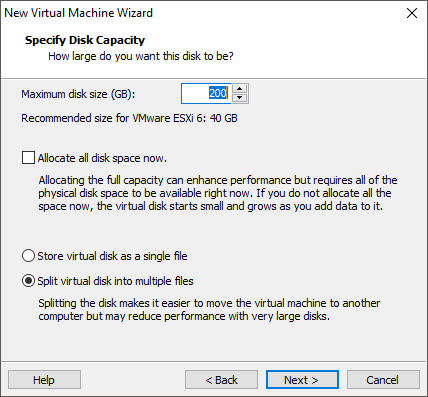
\includegraphics{task1_02_vmwareinstall_08}
          \caption{Setting the maximum disk size for the VM}
          \label{fig:task1:02_vmwarewiz_08}
        \end{figure}
    \end{enumerate}
\end{enumerate}

\subsubsection*{Install ESXi in the new virtual machine}
\begin{enumerate}[resume*=task1methodology]
  \item Start the new ESXi VM in VMware Workstation.
\end{enumerate}

\noindent Upon attempting to start the ESXi VM I received the pop-up window shown in Figure~\ref{fig:task1:02_vmwarewiz_11_issue}.

\begin{figure}[H]
  \centering
  \captionsetup{skip=2pt}
  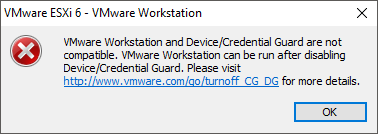
\includegraphics{task1_02_vmwareinstall_11_issue1}
  \caption{VMware issue with Device/Credential Guard}
  \label{fig:task1:02_vmwarewiz_11_issue}
\end{figure}

Following the link provided in the pop-up redirected me to `VMware Knowledge Base Article 2146361'\footnote{\url{https://kb.vmware.com/s/article/2146361}}. Following steps 1 and 2, as detailed on the site under `Resolution' fixed the issue. I have included screenshots of these steps as Figures~\ref{fig:task1:02_vmware_11_res1} and~\ref{fig:task1:02_vmware_11_res2} in the \nameref{app:ancillaryscreenshots} appendix. After completing this resolution process, I was able to start the ESXi VM in VMware Workstation successfully and continued with the task.

\begin{enumerate}[resume*=task1methodology]
  \item Step through the EXSi installer. Notable steps:
    \begin{enumerate}[label=\alph*)]
      \item Select the local storage device.
        \begin{figure}[H]
          \centering
          \captionsetup{skip=2pt}
          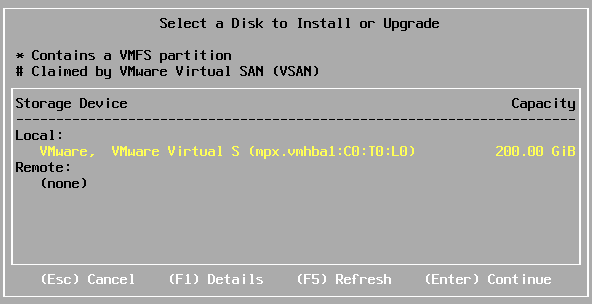
\includegraphics[width=\textwidth]{VMware_ESXi_6-2018-05-08-17-41-37_crop}
          \caption{Selecting the local storage device in the ESXi install}
          \label{fig:task1:esxiinstall_01}
        \end{figure}
      \item Select `United Kingdom' as the keyboard layout.
        \begin{figure}[H]
          \centering
          \captionsetup{skip=2pt}
          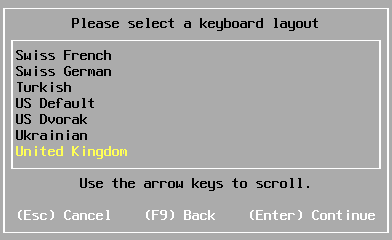
\includegraphics{VMware_ESXi_6-2018-05-08-17-41-48_crop}
          \caption{Selecting the keyboard layout}
          \label{fig:task1:esxiinstall_02}
        \end{figure}
      \item x
    \end{enumerate}
\end{enumerate}
